\documentclass[a4paper,10pt]{jsarticle}

% レイアウト
\setlength{\textwidth}{\fullwidth}
\setlength{\textheight}{39\baselineskip}
\addtolength{\textheight}{\topskip}
\setlength{\voffset}{-0.5in}
\setlength{\headsep}{0.3in}
\pagestyle{myheadings}

% パッケージ
\usepackage[dvipdfmx]{graphicx}
\usepackage{amsmath,amssymb,epsfig}
\usepackage{bm}
\usepackage{ascmac}
\usepackage{pifont}
\usepackage{multirow}
\usepackage{enumerate}
\usepackage{cases}
\usepackage{type1cm}
\usepackage{cancel}
\usepackage{url}
\usepackage{listings,jlisting}
% 大きな中括弧
\usepackage{cases}


% カウンタの設定
\setcounter{section}{0}
\setcounter{subsection}{0}
\setcounter{subsubsection}{0}
\setcounter{equation}{0}

% キャプションの図をFigに変更
\renewcommand{\figurename}{Fig.}
\renewcommand{\tablename}{Tab.}

% 式番号を式(章番号.番号)に
\makeatletter
\renewcommand{\theequation}{\arabic{section}.\arabic{equation}}
\@addtoreset{equation}{section}
\makeatother

% 表紙
\title{知能システム学特論レポート}
\author{
(DL2班)Caffe on Ubuntu\\
}
\date{2015年\ 6月\ 25日}

% ドキュメントの開始
\begin{document}
\maketitle
\section{報告者}
\begin{list}{}{}
 \item 15344203\hspace{0.5cm} 有田 裕太
 \item 15344206\hspace{0.5cm} 緒形 裕太
 \item 15344209\hspace{0.5cm} 株丹 亮
 \item 12104125\hspace{0.5cm} 宮本 和
\end{list}

\section{進行状況}
\begin{itemize}
\item 基本理論の研究
\item 中間層の出力
\end{itemize}

\section{理論研究}
\subsection{人工ニューラルネットワーク}
80年代から90年代にかけて誤差逆伝搬法(back propagation)と呼ばれる多層ニューラルネットワークの学習法の開発をきっかけに多くの研究がなされた.しかし,誤差逆伝搬法では2層程度のニューラルネットワークの学習は行うことができるが,それより多い層をもつニューラルネットワークの学習では様々な問題により上手く学習することが出来ない.

しかし,ディープビリーフネットワーク(deep belief network, DBN)と呼ばれ
るニューラルネットワークに似た多層構造を持つグラフィカルモデルを層ごとに
制約ボルツマンマシン(restricted Boltzmann machine, RBM)という単層ネットワークに分解し,入力層に近い側から順番に教師なしで学習する方法が提案された.この手法で得られたDBMはニューラルネットワークに変換でき,多層であっても学習することが可能となった.目的とするニューラルネットワークの学習前に層ごとに学習を行うことで良い初期値パラメータを求めておくやり方を事前学習(pretraining)という.

その後,同様の結果をより単純な自己符号化器(autoencoder)を使っても多層ニューラルネットワークの事前学習が可能であることが判明した.自己符号化器とは入力に対し,計算される出力が入力になるべく近くなるように訓練されるニューラルネットワークである.自己符号化器を用いて単相ごとに教師なしで学習し,各層のパラメータの初期値を求める.その後,全層のニューラルネットワークを教師ありで学習する.

多層ニューラルネットワークでは,パラメータの初期値をランダムに与えると学習が上手く行えないが,層ごとに教師なし学習を行う事前学習により得られたパラメータを用いることによって上手く学習できることが発見された.

これらの各技術に関して今後深く理解していく.

\begin{figure}[tb]
  \begin{center}
    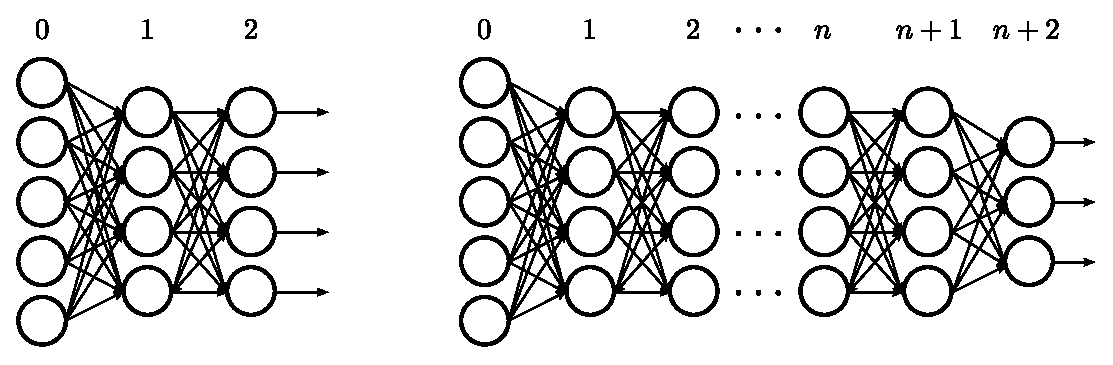
\includegraphics[clip,width=12cm]{./fig/eps/Deep_Learning_concept.eps}
  \end{center}
  \caption{2層のネットワークと多層ネットワークの概念図}
  \label{fig:2層のネットワークと多層ネットワークの概念図}
\end{figure}

\section{プログラム}
\subsection{caffeの基本的なアルゴリズム}
CaffeはCNN(Convolutional Neural Networks)という技法を使っている.CNNは多
層ネットワークで,入力イメージから,特徴を抽出し,オブジェクトの分類を行う.
入力イメージから,低次元の特徴(単純な形状など)を抽出し,処理が進むにつ
れ,高次元の特徴(複雑な形状)を抽出し,画像全体を把握する.低次元の特徴を抽
出することで,オブジェクトを形成する不変の要素を把握できる.更に,CNNに
教育を行うと,その後は自動でオブジェクトを区分でき,コンピュータービジョ
ンの定番技法となっている.

\subsection{中間層の出力}
Caffeで画像を分類する際に中間層でどのような出力なっているかを確認したいと考えているが,現状ではその方法が分かっていない.

\section{今後の課題}
\begin{itemize}
 \item 理論研究を進める.
 \item 中間層の出力,分析する.
\end{itemize}

\end{document}